\documentclass[12pt,a4paper]{article}

\usepackage[utf8]{inputenc}
\usepackage[T1]{fontenc}
\usepackage[brazil]{babel}
\usepackage{lmodern}
\usepackage[a4paper,margin=2.5cm]{geometry}
\usepackage{amsmath,amssymb}
\usepackage{graphicx}
\usepackage{booktabs}
\usepackage{float}
\usepackage{caption}
\usepackage{xcolor}
\usepackage{listings}
\usepackage[hidelinks]{hyperref}

\definecolor{codebg}{RGB}{248,248,248}
\definecolor{codecomment}{RGB}{0,110,0}
\definecolor{codekw}{RGB}{0,0,160}
\definecolor{codestr}{RGB}{160,40,40}

\lstset{
  language=Python,
  basicstyle=\ttfamily\footnotesize,
  backgroundcolor=\color{codebg},
  keywordstyle=\color{codekw}\bfseries,
  commentstyle=\color{codecomment}\itshape,
  stringstyle=\color{codestr},
  numbers=left,
  numberstyle=\tiny\color{gray},
  frame=single,
  breaklines=true,
  showstringspaces=false,
  tabsize=4,
  inputencoding=utf8,
  extendedchars=true,
  literate=
    {á}{{\'a}}1 {à}{{\`a}}1 {ã}{{\~a}}1 {â}{{\^a}}1
    {é}{{\'e}}1 {ê}{{\^e}}1 {í}{{\'i}}1
    {ó}{{\'o}}1 {õ}{{\~o}}1 {ô}{{\^o}}1
    {ú}{{\'u}}1 {ç}{{\c{c}}}1
    {Á}{{\'A}}1 {É}{{\'E}}1 {Í}{{\'I}}1 {Ó}{{\'O}}1 {Ú}{{\'U}}1 {Ç}{{\c{C}}}1
}

% Link do repositório do código
\newcommand{\repositorio}{\url{https://github.com/juliaPamplona/teia-laboratorios/tree/main/lab2}}

\begin{document}

%=====================================================================
% Capa
%=====================================================================
\begin{titlepage}
\centering

\includegraphics[width=0.35\textwidth]{figuras/logo_uepb.png}\\[1.5em]
{\large \textsc{Universidade Estadual da Paraíba}}\\[0.3em]
{\normalsize Disciplina: Tópicos Especiais em Inteligência Artificial}\\[0.3em]
{\normalsize Prof. Robson Pequeno de Sousa}

\vfill

{\LARGE \textbf{Função Discriminante Linear e Algoritmo Perceptron aplicados à base Iris e às tabelas verdade}}\\[1em]
{\large Relatório do Laboratório 02 --- Reconhecimento: função discriminante linear e algoritmo perceptron}

\vfill

{\large Júlia Pamplona}

\vfill

{\large Setembro de 2026}
\end{titlepage}

%=====================================================================
% Resumo
%=====================================================================
\begin{abstract}
Este relatório descreve a implementação, em Python e sem o uso de bibliotecas de aprendizado de máquina, do algoritmo perceptron para duas classes de padrões. O perceptron foi treinado com vetores aumentados, vetor peso inicial nulo e incremento de correção $c = 1$, e aplicado a dois problemas: (i) a base Iris, com 70\% das amostras para treinamento e 30\% para teste (não considerados nesse relatório), nos pares \emph{setosa}~$\times$~\emph{virginica}, \emph{setosa}~$\times$~\emph{versicolor} e \emph{virginica}~$\times$~\emph{versicolor}; e (ii) as tabelas verdade OR, AND e XOR. Com os quatro atributos, os dois pares que envolvem a \emph{setosa} convergiram em duas épocas e classificaram corretamente todo o conjunto de teste, enquanto o par \emph{virginica}~$\times$~\emph{versicolor} não convergiu no limite de 1000 épocas. Com os dois primeiros atributos, as superfícies de separação foram representadas como retas sobre o diagrama de dispersão do conjunto de teste, e o comportamento de convergência se repetiu. Nas tabelas verdade, o algoritmo convergiu para OR e AND e não convergiu para XOR, cujas classes não são linearmente separáveis.

\vspace{1em}
\noindent\textbf{Palavras-chave:} reconhecimento de padrões; função discriminante linear; perceptron; separabilidade linear; base Iris; XOR.
\end{abstract}
\thispagestyle{empty}
\newpage

%=====================================================================
% Sumário
%=====================================================================
\tableofcontents
\thispagestyle{empty}
\newpage

%=====================================================================
\section{Introdução}
%=====================================================================

No laboratório anterior, as funções de decisão foram calculadas diretamente a partir dos vetores protótipos de cada classe. Neste laboratório o caminho é outro: o vetor peso da função discriminante linear é estimado de forma iterativa, a partir do conjunto de treinamento, pelo algoritmo perceptron. Em sua forma mais básica, o perceptron aprende uma função de decisão linear que dicotomiza dois conjuntos de treinamento linearmente separáveis, corrigindo os pesos sempre que um padrão é classificado de forma incorreta.

O objetivo é implementar o perceptron cumprindo os seguintes requisitos:
\begin{enumerate}
  \item Determinar a superfície de separação, utilizando o vetor peso estimado pelo algoritmo, para classificar as classes da base Iris, com 70\% dos dados para treinamento e 30\% para teste;
  \item Utilizar os dois primeiros atributos para definir o diagrama de dispersão e a respectiva superfície de separação, aplicados ao conjunto de teste;
  \item Realizar os itens anteriores para os pares \emph{setosa}~$\times$~\emph{virginica}, \emph{setosa}~$\times$~\emph{versicolor} e \emph{virginica}~$\times$~\emph{versicolor}, verificando se o algoritmo converge;
  \item Usar o perceptron para definir o classificador das tabelas verdade OR, AND e XOR, verificando se os algoritmos convergem;
\end{enumerate}

%=====================================================================
\section{Fundamentação teórica}\label{sec:teoria}
%=====================================================================

\subsection{Função discriminante linear}

Sejam $\omega_i$, $i = 1, 2, \dots, m$, as classes a serem reconhecidas e $\mathbf{x} = (x_1, x_2, \dots, x_n)^t \in \Omega_X$ um vetor de atributos $n$-dimensional. Uma função discriminante $g_i$ é um mapeamento do espaço de atributos $\Omega_X$ para o conjunto dos reais, e cada valor de $i$ está associado a uma única região $R_i$, correspondente a uma classe. Dado $\mathbf{x}$, a atribuição é feita pela regra de decisão
\begin{equation}
  r(\mathbf{x}) = i \iff g_i(\mathbf{x}) > g_j(\mathbf{x}) \quad \forall\, i \neq j,
  \label{eq:regra}
\end{equation}
em que $r(\mathbf{x})$ indica o número da classe de $\mathbf{x}$. A hipersuperfície de decisão que separa duas classes é definida por $g_i(\mathbf{x}) - g_j(\mathbf{x}) = 0$.

No caso linear, a função discriminante tem a forma
\begin{equation}
  g(\mathbf{x}) = \sum_{j=1}^{n} w_j x_j + w_0 = \mathbf{w}^t\mathbf{x} + w_0,
  \label{eq:fdl}
\end{equation}
com $\mathbf{w} = (w_1, w_2, \dots, w_n)^t$ e $w_0$ o peso limiar.

\subsection{Vetores aumentados}

É comum escrever a função discriminante linear em termos de vetores aumentados: acrescenta-se ao vetor de atributos uma componente constante igual a 1 e incorpora-se o peso limiar ao vetor peso. Neste trabalho, a componente constante ocupa a última posição:
\begin{equation}
  \mathbf{y} = (x_1, x_2, \dots, x_n, 1)^t, \qquad
  \mathbf{w} = (w_1, w_2, \dots, w_n, w_{n+1})^t,
  \label{eq:aumentado}
\end{equation}
Assim, $w_{n+1}$ faz o papel do peso limiar $w_0$, e a FDL se reduz a
\begin{equation}
  g(\mathbf{y}) = \mathbf{w}^t\mathbf{y}.
  \label{eq:fdl_aumentada}
\end{equation}
Igualando $g(\mathbf{y}) = 0$, obtém-se a superfície de separação
\begin{equation}
  w_1x_1 + w_2x_2 + \dots + w_nx_n + w_{n+1} = 0,
  \label{eq:superficie}
\end{equation}
que é uma reta quando $n = 2$ e um hiperplano quando $n = 4$.

\subsection{Separabilidade linear}

Duas classes $\omega_1$ e $\omega_2$ são linearmente separáveis se existe um vetor peso tal que
\begin{equation}
  \mathbf{w}^t\mathbf{y} > 0 \ \text{se}\ \mathbf{y} \in \omega_1
  \qquad\text{e}\qquad
  \mathbf{w}^t\mathbf{y} < 0 \ \text{se}\ \mathbf{y} \in \omega_2.
  \label{eq:separavel}
\end{equation}
É sob essa condição que o perceptron converge. Na prática, porém, classes de padrões linearmente separáveis são a exceção, e não a regra.

\subsection{Perceptron para duas classes de padrões}

A resposta do perceptron é baseada na soma ponderada de suas entradas, $g(\mathbf{y}) = \mathbf{w}^t\mathbf{y}$. Os coeficientes $w_i$, $i = 1, 2, \dots, n+1$, chamados pesos, modificam as entradas antes de serem somadas e introduzidas no elemento de limiarização. A função que leva o resultado da soma à saída final do dispositivo, chamada função de ativação, produz $+1$ quando $g(\mathbf{y}) > 0$, indicando que o padrão foi reconhecido como pertencente à classe $\omega_1$, e $-1$ quando $g(\mathbf{y}) < 0$, indicando a classe $\omega_2$.

\subsection{Algoritmo de treinamento}\label{sec:algoritmo}

Considere dois conjuntos de treinamento de vetores aumentados, pertencentes às classes $\omega_1$ e $\omega_2$, e seja $\mathbf{w}(1)$ o vetor inicial de pesos, que pode ser escolhido arbitrariamente. No passo $k$, apresenta-se o padrão $\mathbf{y}(k)$ e aplica-se:
\begin{enumerate}
  \item[i)] se $\mathbf{y}(k) \in \omega_1$ e $\mathbf{w}^t(k)\mathbf{y}(k) \leq 0$, substitua $\mathbf{w}(k)$ por $\mathbf{w}(k+1) = \mathbf{w}(k) + c\,\mathbf{y}(k)$;
  \item[ii)] se $\mathbf{y}(k) \in \omega_2$ e $\mathbf{w}^t(k)\mathbf{y}(k) \geq 0$, substitua $\mathbf{w}(k)$ por $\mathbf{w}(k+1) = \mathbf{w}(k) - c\,\mathbf{y}(k)$;
  \item[iii)] caso contrário, $\mathbf{w}(k+1) = \mathbf{w}(k)$;
\end{enumerate}
sendo $c$ um incremento positivo de correção. Se houver correções durante a passagem pelo conjunto de treinamento, ele é apresentado novamente, e assim sucessivamente, até que uma passagem completa ocorra sem nenhuma correção. Nesse ponto, diz-se que o algoritmo convergiu. Cada apresentação completa do conjunto de treinamento é chamada de \emph{época}.

\subsection{Exemplo}\label{sec:exemplo}

Considere as classes $\omega_1 = \{(0,0)^t, (0,1)^t\}$ e $\omega_2 = \{(1,0)^t, (1,1)^t\}$, representadas pelos vetores aumentados
\[
  \mathbf{y}_1 = (0,0,1)^t,\quad \mathbf{y}_2 = (0,1,1)^t \in \omega_1, \qquad
  \mathbf{y}_3 = (1,0,1)^t,\quad \mathbf{y}_4 = (1,1,1)^t \in \omega_2.
\]
Fazendo $c = 1$ e $\mathbf{w}(1) = \mathbf{0}$ e apresentando os padrões nessa ordem, o algoritmo converge para $\mathbf{w} = (-2, 0, 1)^t$, cuja função de decisão é $g(\mathbf{x}) = -2x_1 + 1$. A fronteira de decisão, obtida com $g(\mathbf{x}) = 0$, é a reta $x_1 = 0{,}5$.

%=====================================================================
\section{Base de dados}
%=====================================================================

A base Iris (arquivo \texttt{Iris data.xls}) contém 150 amostras, 50 de cada espécie: \emph{setosa}, \emph{versicolor} e \emph{virginica}. Cada amostra é descrita por quatro atributos, que formam o vetor de características $\mathbf{x} = (x_1, x_2, x_3, x_4)^t$, na ordem da Tabela~\ref{tab:atributos}.

\begin{table}[H]
\centering
\caption{Atributos da base Iris na ordem do arquivo.}
\label{tab:atributos}
\begin{tabular}{cll}
\toprule
Atributo & Coluna & Descrição \\
\midrule
$x_1$ & \texttt{Sepal length} & comprimento da sépala (cm) \\
$x_2$ & \texttt{Sepal width}  & largura da sépala (cm) \\
$x_3$ & \texttt{Petal length} & comprimento da pétala (cm) \\
$x_4$ & \texttt{Petal width}  & largura da pétala (cm) \\
\bottomrule
\end{tabular}
\end{table}

Os dois primeiros atributos correspondem ao comprimento e à largura da sépala.

%=====================================================================
\section{Metodologia e implementação}
%=====================================================================

O código foi escrito em Python, usando apenas \texttt{pandas} (leitura da planilha), \texttt{numpy} (álgebra vetorial) e \texttt{matplotlib} (gráficos). Nenhuma biblioteca de aprendizado de máquina foi utilizada: a divisão da amostra, o treinamento, a classificação e a acurácia foram implementados manualmente. O código-fonte e as figuras estão disponíveis no repositório \repositorio.

\subsection{Organização do sistema}

O código está organizado em etapas sequenciais, resumidas na Tabela~\ref{tab:etapas}.

\begin{table}[H]
\centering
\caption{Etapas do sistema implementado.}
\label{tab:etapas}
\begin{tabular}{lp{10cm}}
\toprule
Seção & Responsabilidade \\
\midrule
0.1--0.3 & leitura da base, montagem do vetor de características e divisão 70/30 \\
1--2     & formulação do perceptron e funções \texttt{treinar\_perceptron}, \texttt{preparar\_par} e \texttt{prever\_perceptron} \\
3        & treinamento e teste dos três pares de classes com os quatro atributos \\
4        & treinamento com os dois primeiros atributos e diagramas de dispersão com a reta de separação, sobre o conjunto de teste e sobre toda a base \\
5        & histórico de correções por época \\
Parte II & classificadores das tabelas verdade OR, AND e XOR \\
\bottomrule
\end{tabular}
\end{table}

\subsection{Divisão 70\% / 30\%}

Como o perceptron é supervisionado, o vetor peso precisa ser estimado só com o conjunto de treinamento, e a avaliação deve ser feita em amostras que o algoritmo não viu. Para manter as três espécies igualmente representadas, a divisão foi feita dentro de cada classe: as 50 amostras de cada espécie são embaralhadas e separadas em 35 para treinamento e 15 para teste, o que dá 105 e 45 amostras no total. Cada par de classes fica, então, com 70 amostras de treinamento e 30 de teste. A semente aleatória foi fixada em 42 (linha 149) para que os resultados possam ser reproduzidos.

\begin{lstlisting}[firstnumber=120,title=\texttt{pr4\_perceptron\_iris\_colab.py}]
def divisao_treino_teste_estratificada(X, y, percentual_treino=0.70, seed=40):
    rng = np.random.default_rng(seed)

    indices_treino = []
    indices_teste = []

    for classe in np.unique(y):
        indices = np.where(y == classe)[0].copy()
        rng.shuffle(indices)

        n_treino = int(round(len(indices) * percentual_treino))

        indices_treino.extend(indices[:n_treino])
        indices_teste.extend(indices[n_treino:])
\end{lstlisting}

\subsection{Treinamento}\label{sec:treinamento}

O algoritmo da Seção~\ref{sec:algoritmo} está na função \texttt{treinar\_perceptron}. Os padrões são convertidos em vetores aumentados na linha 196, conforme a Eq.~\eqref{eq:aumentado}, e o vetor peso começa nulo, $\mathbf{w}(1) = \mathbf{0}$ (linha 200). O incremento de correção usado foi $c = 1$, passado pelo parâmetro \texttt{taxa\_aprendizado}.

\begin{lstlisting}[firstnumber=193,title=\texttt{pr4\_perceptron\_iris\_colab.py}]
def treinar_perceptron(X_treino_binario, d_treino, taxa_aprendizado=1.0, max_epocas=1000):

    # Adiciona o termo de bias: 1
    X_aumentado = np.c_[X_treino_binario, np.ones(len(X_treino_binario))]

    # Vetor peso inicial w(1):
    # todos os pesos começam em zero.
    w = np.zeros(X_aumentado.shape[1])

    erros_por_epoca = []

    for epoca in range(1, max_epocas + 1):
        erros = 0

        for x, d in zip(X_aumentado, d_treino):
            g = np.dot(w, x)

            # Se o padrão não foi corretamente classificado,
            # atualiza os pesos.
            if d * g <= 0:
                w = w + taxa_aprendizado * d * x
                erros += 1

        erros_por_epoca.append(erros)

        # Se não houve nenhum erro, houve convergência.
        if erros == 0:
            return w, epoca, True, erros_por_epoca

    return w, max_epocas, False, erros_por_epoca
\end{lstlisting}

Em vez de tratar as regras i) e ii) separadamente, cada padrão de treinamento recebe uma resposta desejada $d$, igual a $+1$ para $\omega_1$ e $-1$ para $\omega_2$ (função \texttt{preparar\_par}), e as duas regras passam a ser escritas como uma só (linhas 212--213):
\[
  \text{se}\ d\,\mathbf{w}^t(k)\mathbf{y}(k) \leq 0, \quad \mathbf{w}(k+1) = \mathbf{w}(k) + c\,d\,\mathbf{y}(k).
\]
Com $d = +1$, essa expressão é exatamente a regra i); com $d = -1$, a condição vira $\mathbf{w}^t(k)\mathbf{y}(k) \geq 0$ e a correção vira $\mathbf{w}(k) - c\,\mathbf{y}(k)$, que é a regra ii). Quando a condição não é satisfeita, o vetor peso não muda, como na regra iii).

Ao final de cada época, a função verifica se houve alguma correção. Se não houve (linhas 219--220), todos os padrões de treinamento satisfazem a Eq.~\eqref{eq:separavel} e o treinamento termina. Como em classes não linearmente separáveis as correções nunca param, foi preciso definir um limite de 1000 épocas; ao atingi-lo, o treinamento é interrompido e registrado como não convergente. A função também devolve o número de correções de cada época, usado na Seção~\ref{sec:convergencia}.

O valor de $c$ não altera os resultados quando $\mathbf{w}(1) = \mathbf{0}$: nesse caso, todo vetor peso gerado pelo algoritmo é múltiplo de $c$, e a condição de correção não depende da escala de $\mathbf{w}$. Por isso foi mantido $c = 1$.

Antes de aplicar o algoritmo à base Iris, a função foi testada com os padrões do exemplo da Seção~\ref{sec:exemplo}, na mesma ordem de apresentação, com $c = 1$ e $\mathbf{w}(1) = \mathbf{0}$. O vetor obtido foi $\mathbf{w} = (-2, 0, 1)^t$, igual ao do exemplo, o que confirmou que a implementação estava correta.

\subsection{Classificação e superfície de separação}

Com o vetor peso estimado, a função \texttt{prever\_perceptron} calcula $g(\mathbf{y}) = \mathbf{w}^t\mathbf{y}$ para cada amostra de teste e aplica a função de ativação:

\begin{lstlisting}[firstnumber=234,title=\texttt{pr4\_perceptron\_iris\_colab.py}]
def prever_perceptron(X_amostras, w, classe_positiva, classe_negativa):
    X_aumentado = np.c_[X_amostras, np.ones(len(X_amostras))]
    g = X_aumentado @ w

    previsoes = np.where(
        g >= 0,
        classe_positiva,
        classe_negativa
    )

    return previsoes, g
\end{lstlisting}

A função de ativação está definida para $g > 0$ e $g < 0$, mas um padrão pode cair exatamente sobre a superfície ($g = 0$). Para esse caso, optou-se por atribuir o padrão à classe $\omega_1$. No treinamento, $g = 0$ conta como erro (condição $\leq 0$); assim, quando há convergência, nenhum padrão de treinamento fica sobre a superfície.

Para cada par, o programa imprime a acurácia no teste e a superfície de separação na forma da Eq.~\eqref{eq:superficie}, montada diretamente a partir do vetor peso (linhas 311--312).

\subsection{Pares de classes da base Iris}

Como o perceptron separa apenas duas classes, cada par recebeu um perceptron próprio, treinado somente com as amostras de treinamento das duas espécies envolvidas. A primeira classe de cada par foi tratada como $\omega_1$ (saída $+1$) e a segunda como $\omega_2$ (saída $-1$): \emph{setosa}~$\times$~\emph{virginica}, \emph{setosa}~$\times$~\emph{versicolor} e \emph{virginica}~$\times$~\emph{versicolor}.

O classificador principal usa os quatro atributos, e sua superfície de separação é um hiperplano em $\mathbb{R}^4$, impossível de representar em um diagrama de dispersão. Para a visualização, a função \texttt{plotar\_perceptron\_2d} treina um segundo perceptron por par, agora apenas com os dois primeiros atributos $(x_1, x_2)$. A Eq.~\eqref{eq:superficie} se torna então a reta
\begin{equation}
  w_1x_1 + w_2x_2 + w_3 = 0
  \quad\Longrightarrow\quad
  x_2 = -\frac{w_1x_1 + w_3}{w_2}, \qquad w_2 \neq 0,
  \label{eq:reta}
\end{equation}
que é desenhada sobre as amostras do conjunto de teste. Se $w_2 = 0$, desenha-se a reta vertical $x_1 = -w_3/w_1$. Quando o algoritmo não converge, a reta exibida é a do vetor peso da última época, em linha tracejada.

Na primeira versão dos gráficos, a reta do par \emph{virginica}~$\times$~\emph{versicolor}, quase vertical, esticava o eixo vertical até valores entre $-20$ e $35$ e espremia os pontos em uma faixa estreita. Por isso, o eixo vertical passou a ser limitado ao intervalo dos dados (linha 405).

\subsection{Tabelas verdade}

Nas tabelas verdade, os padrões são os quatro pares de entrada $(x_1, x_2) \in \{0,1\}^2$, e a saída lógica foi convertida em resposta desejada: saída 1 corresponde a $d = +1$ (classe $\omega_1$) e saída 0 a $d = -1$ (classe $\omega_2$). Os padrões são apresentados na ordem $(1,1)$, $(1,0)$, $(0,1)$, $(0,0)$, e o treinamento usa a mesma função e os mesmos parâmetros da base Iris:

\begin{lstlisting}[firstnumber=559,title=\texttt{pr4\_perceptron\_iris\_colab.py}]
def executar_tabela_verdade(nome, saidas_logicas):
    # Converte 1 -> +1 e 0 -> -1
    d = np.where(saidas_logicas == 1, 1, -1)

    w, epocas, convergiu, historico = treinar_perceptron(
        X_logica,
        d,
        taxa_aprendizado=1.0,
        max_epocas=1000
    )

    X_aumentado = np.c_[X_logica, np.ones(len(X_logica))]
    g = X_aumentado @ w

    saidas_preditas = np.where(g >= 0, 1, 0)
\end{lstlisting}

%=====================================================================
\section{Resultados}\label{sec:resultados}
%=====================================================================

\subsection{Base Iris com os quatro atributos}

A Tabela~\ref{tab:iris4d} mostra o resultado dos três perceptrons treinados com o vetor de características completo.

\begin{table}[H]
\centering
\caption{Perceptron com os quatro atributos (70 amostras de treinamento e 30 de teste por par).}
\label{tab:iris4d}
\begin{tabular}{lccc}
\toprule
Par ($\omega_1 \times \omega_2$) & Convergiu? & Épocas & Acertos no teste \\
\midrule
\emph{setosa} $\times$ \emph{virginica}     & sim & 2    & 30/30 (100\%) \\
\emph{setosa} $\times$ \emph{versicolor}    & sim & 2    & 30/30 (100\%) \\
\emph{virginica} $\times$ \emph{versicolor} & não & 1000 & 29/30 (96,67\%) \\
\bottomrule
\end{tabular}
\end{table}

Substituindo os vetores peso estimados na Eq.~\eqref{eq:superficie}, chega-se às seguintes superfícies de separação:
\begin{align*}
\textit{setosa} \times \textit{virginica}:&\quad 1{,}7x_1 + 4{,}3x_2 - 7{,}1x_3 - 3{,}6x_4 + 1{,}0 = 0\\
\textit{setosa} \times \textit{versicolor}:&\quad 1{,}8x_1 + 6{,}2x_2 - 8{,}6x_3 - 3{,}9x_4 + 1{,}0 = 0\\
\textit{virginica} \times \textit{versicolor}:&\quad -75{,}0x_1 - 133{,}5x_2 + 153{,}5x_3 + 202{,}4x_4 - 239{,}0 = 0
\end{align*}

Os pares com a \emph{setosa} precisaram de apenas uma época com correções (5 e 9, respectivamente); na segunda época, todo o conjunto de treinamento já foi classificado corretamente. Os coeficientes negativos de $x_3$ e $x_4$ fazem sentido: $g(\mathbf{y}) > 0$ corresponde à \emph{setosa}, que tem pétalas bem menores que as das outras espécies.

Já no par \emph{virginica}~$\times$~\emph{versicolor}, nenhuma das 1000 épocas terminou sem correções; mesmo no fim do treinamento, ainda ocorriam de 2 a 6 correções por época. O hiperplano apresentado acima é, portanto, apenas o da época 1000, e não uma solução convergida. Mesmo assim, ele acertou 29 das 30 amostras de teste.

\subsection{Base Iris com os dois primeiros atributos}

A Tabela~\ref{tab:iris2d} reúne as retas obtidas com o comprimento e a largura da sépala, e as Figuras~\ref{fig:sv}, \ref{fig:sver} e~\ref{fig:vver} mostram essas retas sobre o diagrama de dispersão do conjunto de teste.

\begin{table}[H]
\centering
\caption{Perceptron com os dois primeiros atributos (sépala). Os acertos no teste são as amostras que ficaram do lado correto da reta.}
\label{tab:iris2d}
\begin{tabular}{llccc}
\toprule
Par ($\omega_1 \times \omega_2$) & Reta de separação & Convergiu? & Épocas & Teste \\
\midrule
\emph{setosa} $\times$ \emph{virginica}     & $-43{,}3x_1 + 69{,}6x_2 + 36{,}0 = 0$  & sim & 99   & 29/30 \\
\emph{setosa} $\times$ \emph{versicolor}    & $-76{,}9x_1 + 98{,}4x_2 + 120{,}0 = 0$ & sim & 770  & 30/30 \\
\emph{virginica} $\times$ \emph{versicolor} & $25{,}1x_1 + 1{,}6x_2 - 171{,}0 = 0$   & não & 1000 & 19/30 \\
\bottomrule
\end{tabular}
\end{table}

\begin{figure}[H]
\centering
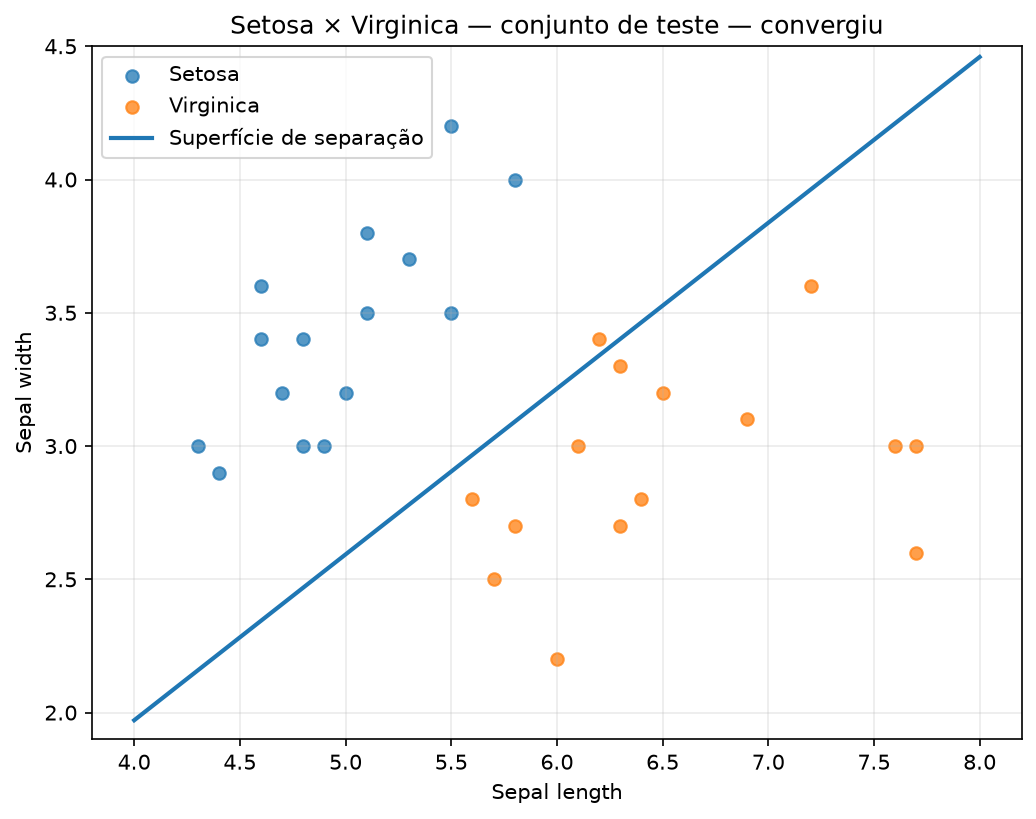
\includegraphics[width=0.72\textwidth]{figuras/sv_teste.png}
\caption{\emph{Setosa} $\times$ \emph{virginica}: conjunto de teste e reta de separação $-43{,}3x_1 + 69{,}6x_2 + 36{,}0 = 0$.}
\label{fig:sv}
\end{figure}

Para \emph{setosa}~$\times$~\emph{virginica} (Figura~\ref{fig:sv}), o algoritmo convergiu em 99 épocas, e a reta separa todas as amostras de treinamento. No teste, porém, uma amostra de \emph{virginica}, com $(x_1, x_2) = (6{,}2;\ 3{,}4)$, ficou do lado da \emph{setosa}. A convergência garante a separação do conjunto de treinamento, mas não de amostras novas.

\begin{figure}[H]
\centering
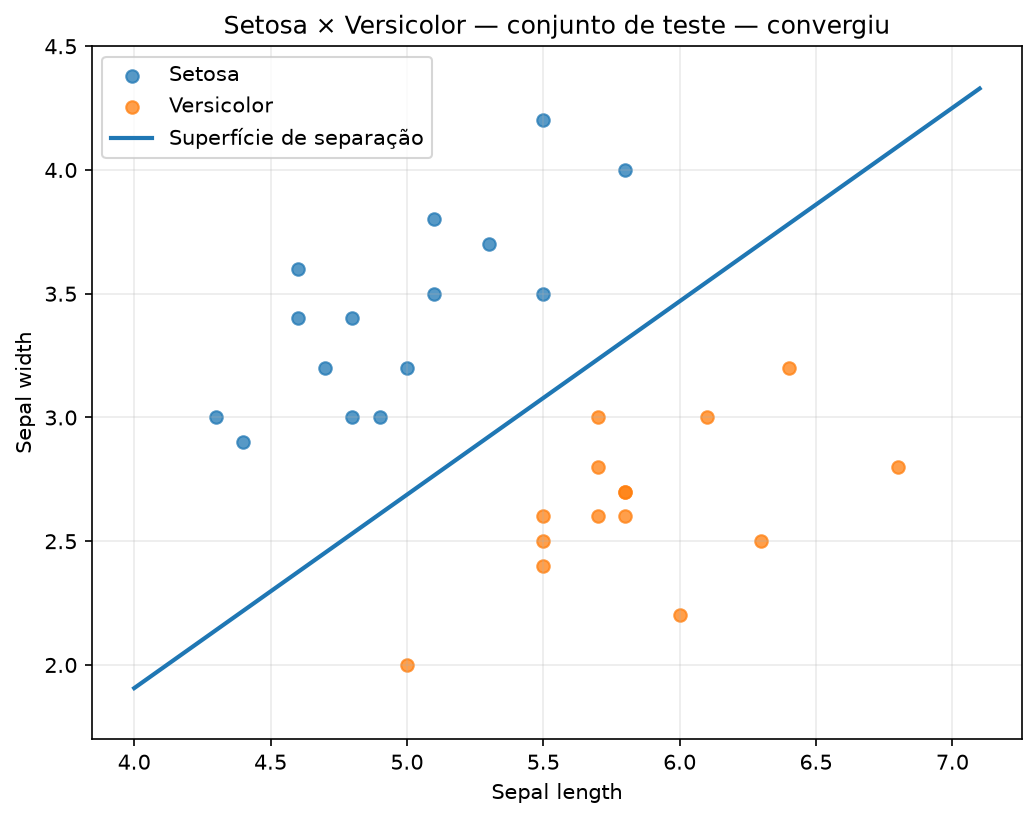
\includegraphics[width=0.72\textwidth]{figuras/sver_teste.png}
\caption{\emph{Setosa} $\times$ \emph{versicolor}: conjunto de teste e reta de separação $-76{,}9x_1 + 98{,}4x_2 + 120{,}0 = 0$.}
\label{fig:sver}
\end{figure}

Em \emph{setosa}~$\times$~\emph{versicolor} (Figura~\ref{fig:sver}) também houve convergência, mas só após 770 épocas, e a reta separou todas as amostras de teste. A demora se explica pela proximidade entre as duas nuvens no plano da sépala: como a folga entre elas é pequena, o algoritmo faz muitas correções até chegar a uma reta que separe todos os pontos.

\begin{figure}[H]
\centering
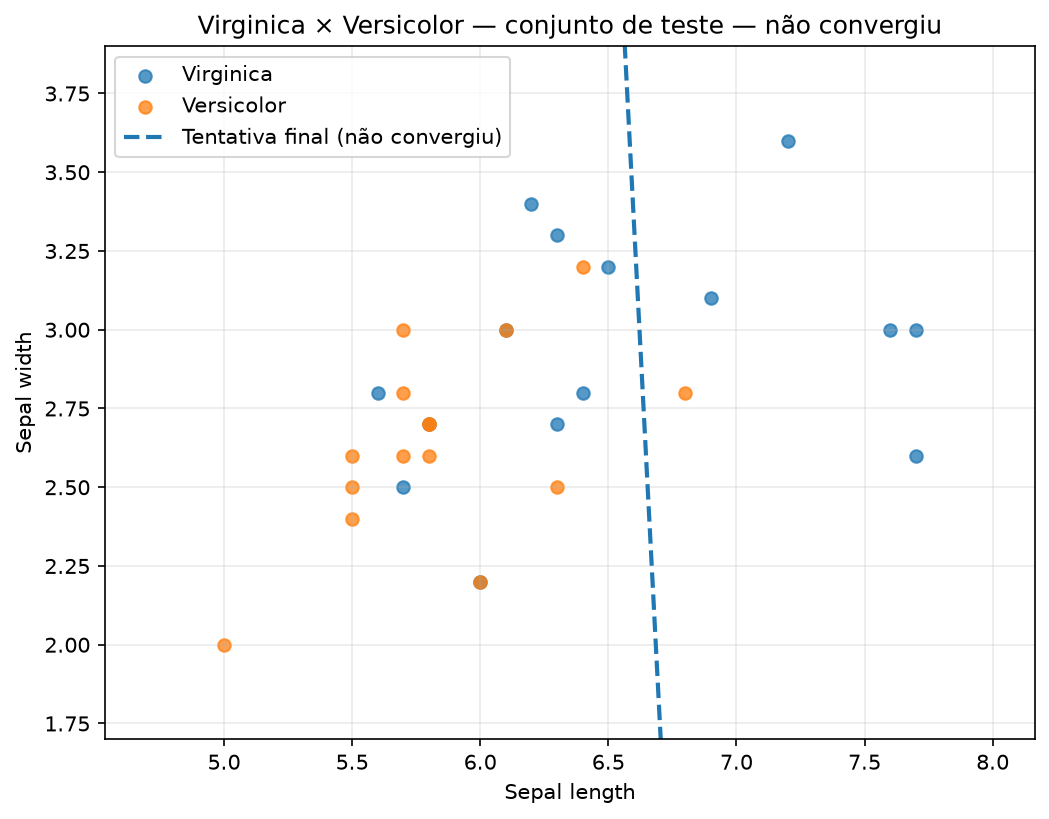
\includegraphics[width=0.72\textwidth]{figuras/vver_teste.png}
\caption{\emph{Virginica} $\times$ \emph{versicolor}: conjunto de teste e reta da época 1000, $25{,}1x_1 + 1{,}6x_2 - 171{,}0 = 0$, tracejada porque o algoritmo não convergiu.}
\label{fig:vver}
\end{figure}

No par \emph{virginica}~$\times$~\emph{versicolor} (Figura~\ref{fig:vver}), as nuvens de pontos se misturam no plano da sépala, e não há reta que deixe todas as amostras de uma espécie de um lado e todas as da outra do lado oposto. O algoritmo não convergiu, e a reta da última época, quase vertical em torno de $x_1 \approx 6{,}6$, deixou 11 das 30 amostras de teste do lado errado.

\subsection{Convergência}\label{sec:convergencia}

A Figura~\ref{fig:erros} mostra quantas correções ocorreram em cada época do treinamento com os dois primeiros atributos.

\begin{figure}[H]
\centering
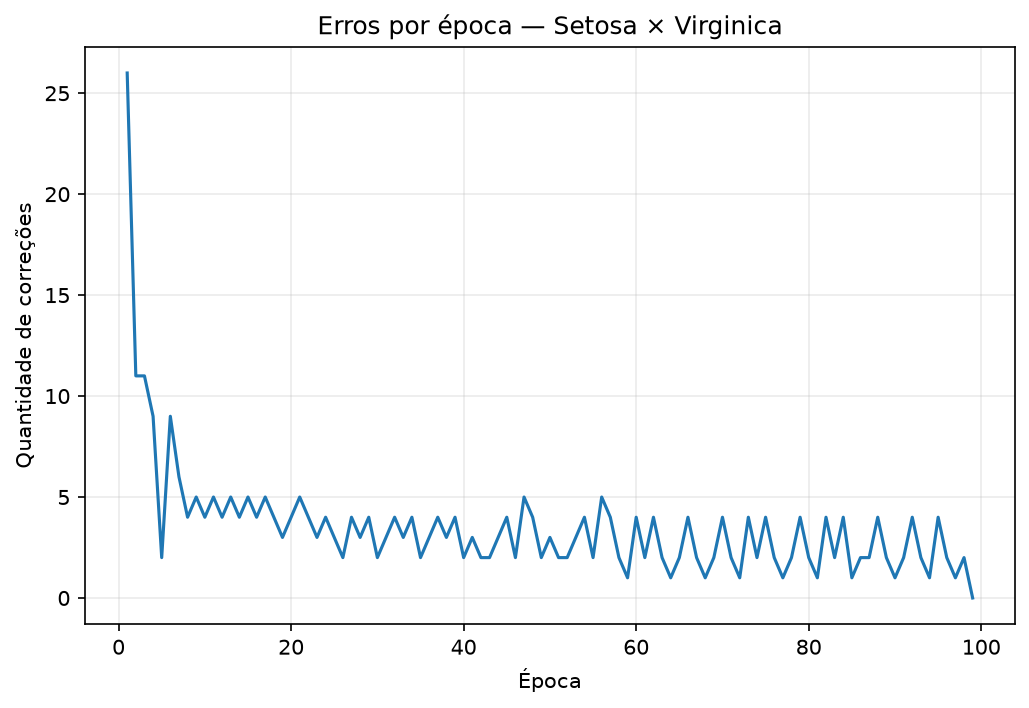
\includegraphics[width=0.49\textwidth]{figuras/erros_sv.png}\hfill
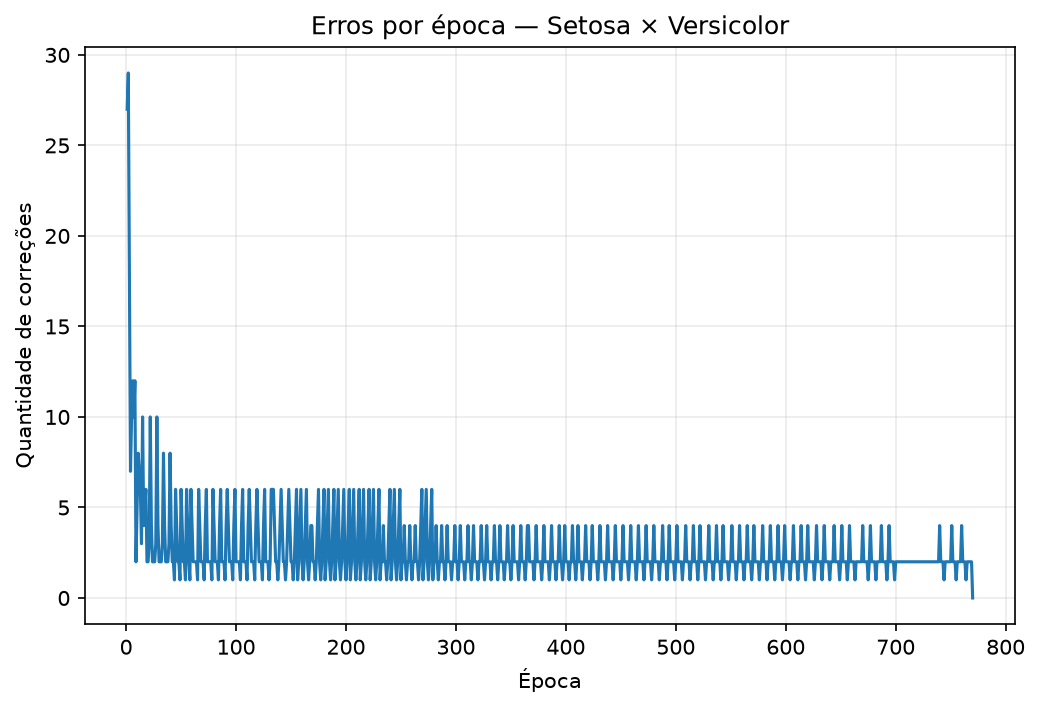
\includegraphics[width=0.49\textwidth]{figuras/erros_sver.png}\\[0.5em]
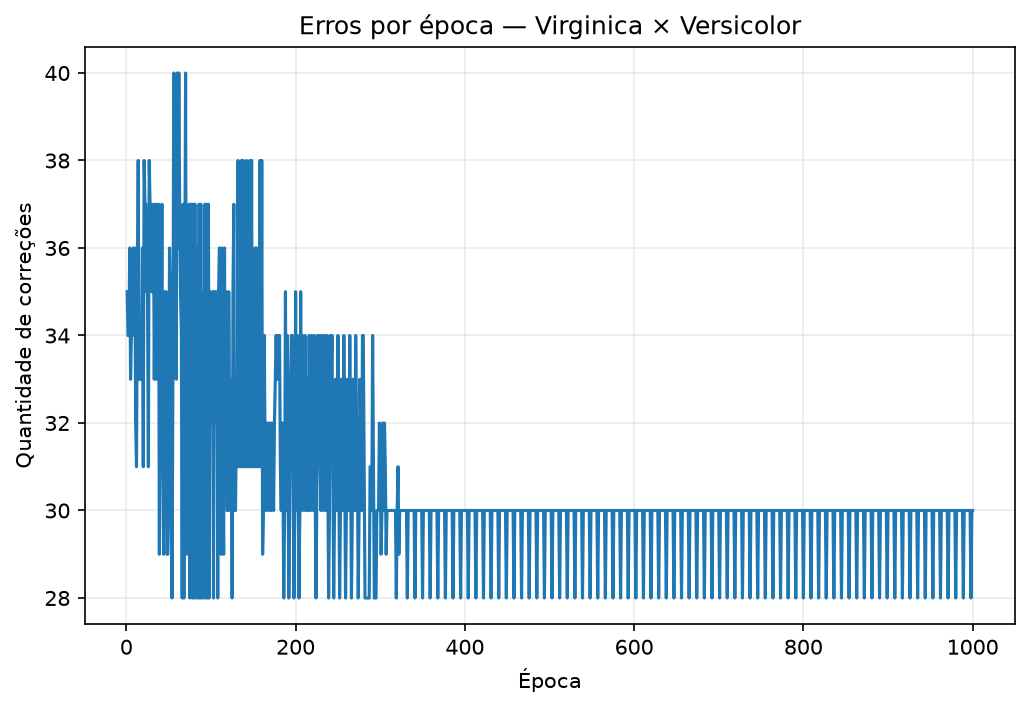
\includegraphics[width=0.49\textwidth]{figuras/erros_vver.png}
\caption{Número de correções por época com os dois primeiros atributos: \emph{setosa} $\times$ \emph{virginica} (acima, à esquerda), \emph{setosa} $\times$ \emph{versicolor} (acima, à direita) e \emph{virginica} $\times$ \emph{versicolor} (abaixo).}
\label{fig:erros}
\end{figure}

Nos pares com a \emph{setosa}, as correções vão diminuindo até chegar a zero, quando o algoritmo converge. Em \emph{virginica}~$\times$~\emph{versicolor} isso não acontece: depois de uma fase inicial com 28 a 40 correções por época, o algoritmo passa a alternar entre 28 e 30 correções e permanece assim até a época 1000.

Respondendo à pergunta do enunciado, o algoritmo não converge para o par \emph{virginica}~$\times$~\emph{versicolor}. Isso vale tanto para os quatro atributos quanto para os dois primeiros: em nenhum dos casos foi encontrado um vetor peso que satisfizesse a Eq.~\eqref{eq:separavel} para todo o conjunto de treinamento, o que indica que essas duas classes não são linearmente separáveis. Nos pares com a \emph{setosa}, ao contrário, houve convergência nas duas representações.

\subsection{Tabelas verdade}

A Tabela~\ref{tab:logica} resume o treinamento para as três funções lógicas.

\begin{table}[H]
\centering
\caption{Perceptron aplicado às tabelas verdade.}
\label{tab:logica}
\begin{tabular}{lcccc}
\toprule
Função & Convergiu? & Épocas & Vetor peso $\mathbf{w}$ & Superfície de separação \\
\midrule
OR  & sim & 5    & $(2, 2, -1)^t$ & $2x_1 + 2x_2 - 1 = 0$ \\
AND & sim & 10   & $(2, 3, -4)^t$ & $2x_1 + 3x_2 - 4 = 0$ \\
XOR & não & 1000 & ---            & --- \\
\bottomrule
\end{tabular}
\end{table}

Para OR e AND, a saída do classificador coincide com a saída desejada nas quatro combinações de entrada (Tabela~\ref{tab:or_and}): $g(\mathbf{x})$ é positivo sempre que a saída lógica é 1 e negativo sempre que é 0.

\begin{table}[H]
\centering
\caption{Saída dos classificadores OR, $g(\mathbf{x}) = 2x_1 + 2x_2 - 1$, e AND, $g(\mathbf{x}) = 2x_1 + 3x_2 - 4$.}
\label{tab:or_and}
\begin{tabular}{cc|ccc|ccc}
\toprule
 & & \multicolumn{3}{c|}{OR} & \multicolumn{3}{c}{AND} \\
$x_1$ & $x_2$ & Desejada & $g(\mathbf{x})$ & Saída & Desejada & $g(\mathbf{x})$ & Saída \\
\midrule
1 & 1 & 1 & $3$  & 1 & 1 & $1$  & 1 \\
1 & 0 & 1 & $1$  & 1 & 0 & $-2$ & 0 \\
0 & 1 & 1 & $1$  & 1 & 0 & $-1$ & 0 \\
0 & 0 & 0 & $-1$ & 0 & 0 & $-4$ & 0 \\
\bottomrule
\end{tabular}
\end{table}

No XOR, o algoritmo não converge. Todas as quatro apresentações de cada época geram correção, e o vetor peso volta a ser nulo no fim de cada época. A Tabela~\ref{tab:xor} mostra a primeira época: como ela termina em $\mathbf{w} = \mathbf{0}$, que é o próprio vetor inicial, as épocas seguintes repetem exatamente a mesma sequência, e o algoritmo fica preso nesse ciclo até o limite de 1000 épocas. O vetor final é, por isso, $\mathbf{w} = (0, 0, 0)^t$, com $g(\mathbf{x}) = 0$ para todas as entradas, e nenhuma superfície de separação é obtida.

\begin{table}[H]
\centering
\caption{Primeira época do perceptron para o XOR ($c = 1$, $\mathbf{w}(1) = \mathbf{0}$).}
\label{tab:xor}
\begin{tabular}{cccccc}
\toprule
$k$ & $\mathbf{y}(k)$ & $d$ & $\mathbf{w}^t(k)\mathbf{y}(k)$ & Correção & $\mathbf{w}(k+1)$ \\
\midrule
1 & $(1,1,1)^t$ & $-1$ & $0$  & $\mathbf{w}(k) - \mathbf{y}(k)$ & $(-1,-1,-1)^t$ \\
2 & $(1,0,1)^t$ & $+1$ & $-2$ & $\mathbf{w}(k) + \mathbf{y}(k)$ & $(0,-1,0)^t$ \\
3 & $(0,1,1)^t$ & $+1$ & $-1$ & $\mathbf{w}(k) + \mathbf{y}(k)$ & $(0,0,1)^t$ \\
4 & $(0,0,1)^t$ & $-1$ & $1$  & $\mathbf{w}(k) - \mathbf{y}(k)$ & $(0,0,0)^t$ \\
\bottomrule
\end{tabular}
\end{table}

O motivo é que as classes do XOR não são linearmente separáveis. Pela Eq.~\eqref{eq:separavel}, um vetor $\mathbf{w} = (w_1, w_2, w_3)^t$ que as separasse teria de satisfazer
\[
  w_1 + w_3 > 0, \qquad w_2 + w_3 > 0, \qquad w_1 + w_2 + w_3 < 0, \qquad w_3 < 0.
\]
Somando as duas primeiras desigualdades, obtém-se $w_1 + w_2 + w_3 > -w_3 > 0$, o que contradiz a terceira. Não existe, portanto, reta capaz de separar as saídas 1 das saídas 0.

%=====================================================================
\section{Discussão}
%=====================================================================

Os experimentos se comportaram como a teoria prevê: o perceptron converge quando as classes são linearmente separáveis e segue corrigindo o vetor peso indefinidamente quando não são. A \emph{setosa} se separa linearmente das outras duas espécies tanto com os quatro atributos quanto apenas com a sépala, enquanto \emph{virginica} e \emph{versicolor} não se separam em nenhuma das duas representações. Nas tabelas verdade acontece o mesmo: OR e AND são linearmente separáveis, o XOR não. Fica claro que, em problemas reais, encontrar classes linearmente separáveis é mais exceção do que regra.

A escolha dos atributos também pesou no tempo de convergência. Com os quatro atributos, os pares com a \emph{setosa} convergiram em duas épocas; usando só a sépala, foram necessárias 99 e 770. Os coeficientes de maior módulo nos hiperplanos estão em $x_3$ e $x_4$, o que indica que são as medidas da pétala que mais afastam as classes. Sem elas, as nuvens ficam mais próximas e a busca pela reta de separação demora mais.

Outro ponto é o significado do vetor peso quando não há convergência. Como ele continua sendo corrigido a cada época, o resultado final depende de quando o treinamento é interrompido. No par \emph{virginica}~$\times$~\emph{versicolor} com quatro atributos, o vetor da época 1000 acertou 29 das 30 amostras de teste, mas nada garante esse desempenho: outra época de parada poderia levar a um hiperplano diferente. Com a sépala, onde a sobreposição é maior, a reta final acertou apenas 19 das 30.

Por fim, vale registrar algumas limitações. Os resultados vêm de uma única divisão 70/30 com semente fixa, e cada par tem só 30 amostras de teste, de modo que um único erro já representa cerca de 3,3 pontos percentuais. Além disso, a não convergência foi observada dentro de um limite de 1000 épocas. No XOR, a impossibilidade de separação foi demonstrada algebricamente; em \emph{virginica}~$\times$~\emph{versicolor}, a evidência é experimental, dada pela persistência de correções em todas as épocas.

%=====================================================================
\section{Conclusão}
%=====================================================================

O algoritmo perceptron para duas classes foi implementado sem bibliotecas de aprendizado de máquina, usando a função discriminante linear em termos de vetores aumentados, vetor peso inicial nulo e a correção $\mathbf{w}(k+1) = \mathbf{w}(k) \pm c\,\mathbf{y}(k)$ a cada padrão classificado incorretamente. A implementação foi conferida com o exemplo da Seção~\ref{sec:exemplo}, reproduzindo o vetor $\mathbf{w} = (-2, 0, 1)^t$.

Na base Iris, com 70\% das amostras para treinamento e 30\% para teste, o algoritmo convergiu para os pares \emph{setosa}~$\times$~\emph{virginica} e \emph{setosa}~$\times$~\emph{versicolor}, e as superfícies de separação obtidas com os quatro atributos classificaram corretamente todo o conjunto de teste. Para \emph{virginica}~$\times$~\emph{versicolor}, o algoritmo não converge, já que essas classes não são linearmente separáveis. Os diagramas de dispersão do conjunto de teste, feitos com os dois primeiros atributos, deixam essa diferença visível: nos pares com a \emph{setosa} a reta separa as classes, enquanto no par \emph{virginica}~$\times$~\emph{versicolor} as nuvens se sobrepõem.

Nas tabelas verdade, o perceptron levou aos classificadores $2x_1 + 2x_2 - 1 = 0$, para o OR, e $2x_1 + 3x_2 - 4 = 0$, para o AND, ambos reproduzindo suas tabelas. Para o XOR, o algoritmo não converge, pois nenhuma reta separa as saídas 1 das saídas 0; trata-se do caso clássico em que um perceptron simples não é suficiente.

%=====================================================================
% Referências
%=====================================================================
\begin{thebibliography}{9}

\bibitem{sousa}
SOUSA, R. P. de. \textbf{Reconhecimento: função discriminante linear e algoritmo perceptron}. Material didático da disciplina Tópicos Especiais em Inteligência Artificial. Campina Grande: Universidade Estadual da Paraíba, 2026.

\bibitem{gonzalez}
GONZALEZ, R. C.; WOODS, R. E. \textbf{Digital Image Processing}. 4. ed. New York: Pearson, 2018.

\bibitem{repo}
PAMPLONA, J. \textbf{Laboratório 02: função discriminante linear e algoritmo perceptron aplicados à base Iris e às tabelas verdade}. Repositório de código-fonte, 2026. Disponível em: \repositorio. Acesso em: out. 2026.

\end{thebibliography}

\end{document}
